% HINT: add option aspectratio=169 for 16:9 aspect ratio
% HINT: add 'handout' to activate handout mode (without overlays for printing)
\documentclass[t,german,aspectratio=169]{beamer}

% include package import and macro defintions
% Math
\usepackage{amsmath}
\usepackage{upgreek}

% Miscelaneous
\usepackage{pgfpages}
\usepackage{csquotes}
\usepackage{placeins}

% Captions
\usepackage[labelformat=empty]{caption}

% Colors
\usepackage{xcolor}

% Requirements
\RequirePackage{tikz}
\usetikzlibrary{calc}
\usetikzlibrary{arrows,shapes,positioning}

% For \smiley{} and \frowney{}
\usepackage{wasysym}

% Pseudocode
\usepackage[vlined, linesnumbered, ruled]{algorithm2e}
\SetKwComment{Comment}{/* }{*/}
\SetKwInput{KwData}{Input}
\SetKwInput{KwResult}{Output}
\IncMargin{1.5em}

% nice icons
%\usepackage{fontawesome}

% IMPORTANT NOTE: outputdir needs to be equal to output/aux dir of xelatex
%\usepackage[outputdir=output]{minted}
\usepackage{appendixnumberbeamer}

% Tables
\usepackage{booktabs}
\usepackage{multicol}
\usepackage{multirow}
\usepackage{colortbl}

% Date formatting
\usepackage[short,nodayofweek]{datetime}

% Für Vektoren
\newcommand{\myvec}[1]{\ensuremath{\begin{pmatrix}#1\end{pmatrix}}}
\def\spvec#1{\left(\vcenter{\halign{\hfil$##$\hfil\cr \spvecA#1;;}}\right)}
\def\spvecA#1;{\if;#1;\else #1\cr \expandafter \spvecA \fi}

% Hyperlinks
\definecolor{citeblue}{rgb}{0,0.3,0.55}
\RequirePackage{hyperref}
\hypersetup{colorlinks,linkcolor={lightgray},citecolor={citeblue},urlcolor={citeblue}}
\let\oldciteauthor=\citeauthor
\def\citeauthor#1{\hypersetup{citecolor=white}\oldciteauthor{#1}}

% Added
\usepackage{circuitikz}
\usepackage{grfext}

% Reelle, Natürliche, Ganze, Rationale Zahlen
\newcommand{\R}{\ensuremath{\mathbb{R}}}
\newcommand{\N}{\ensuremath{\mathbb{N}}}
\newcommand{\Z}{\ensuremath{\mathbb{Z}}}
\newcommand{\Q}{\ensuremath{\mathbb{Q}}}

\usetikzlibrary{decorations.pathreplacing,calc}
\newcommand{\tikzmark}[1]{\tikz[overlay,remember picture] \node (#1) {};}

\newcommand*{\AddNote}[5]{%
	\begin{tikzpicture}[overlay, remember picture]
		\draw [decoration={brace,amplitude=0.5em},decorate,ultra thick,color=#4]
		($(#3)!(#2.south)!($(#3)-(0,1)$)$) --
		($(#3)!(#1.north)!($(#3)-(0,1)$)$)
		node [align=center, text width=0.5cm, pos=0.5, anchor=east] {#5};
	\end{tikzpicture}
}%

\usepackage{algpseudocode}% http://ctan.org/pkg/algorithmicx
%\usepackage{algorithm}% http://ctan.org/pkg/algorithm

% captions for subfigures.
\usepackage{subcaption}


% Clever references.
\usepackage{hyperref}
\usepackage{cleveref}
\usepackage{amssymb}
%% commenting macros

% use this to hide larger blocks of material:
\usepackage{xcolor}
\usepackage{amsmath,amssymb}

% Define colors for authors
\definecolor{johannescolor}{rgb}{0.2,0.6,0.6}
\definecolor{danjecolor}{rgb}{0,0.7,0}

% Define colors for general macros
\definecolor{todocolor}{rgb}{0.9,0.1,0.1}
\definecolor{changedcolor}{rgb}{0.42,0.27,0.57}
\definecolor{addedcolor}{rgb}{0.867,0.176,0.361}
\definecolor{sourcecolor}{rgb}{0.25,0.4,0.7}

% General comment macro
\newcommand{\nbc}[3]{
    {\colorbox{#3}{\bfseries\sffamily\scriptsize\textcolor{white}{#1}}}
    {\textcolor{#3}{\sf\small$\blacktriangleright$\textit{#2}$\blacktriangleleft$}}
}
\newcommand{\cbs}[3]{
    {\colorbox{#2}{\bfseries\sffamily\scriptsize\textcolor{white}{#1}}}
}
  
% Define individual comments for authors
\newcommand{\johannes}[1]{\nbc{Johannes}{#1}{johannescolor}}
\newcommand{\danje}[1]{\nbc{Danje}{#1}{danjecolor}}

% Define general helper macros
\newcommand{\todo}[1]{\nbc{TODO}{#1}{todocolor}}
\newcommand{\changed}[1]{\nbc{CHANGED}{#1}{changedcolor}}
\newcommand{\added}[1]{\nbc{ADDED}{#1}{addedcolor}}
\newcommand{\source}[1]{\cbs{SOURCE MISSING}{sourcecolor}}

\newcommand{\redacted}[1]{\emph{[anonymized for review]}}
%\renewcommand{\redacted}[1]{#1}

% Use this to temporarily hide reviewing comments, todos, etc.:
%  \renewcommand{\jane}[1]{}
%  \renewcommand{\john}[1]{}

% Use this to make "changed" items appear normal:
%\renewcommand{\changed}[1]{#1}
%\renewcommand{\added}[1]{#1}
%\renewcommand{\todo}[1]{}

%% end commenting macros


% add (multiple) bibliography sources for biblatex


% Set authorinfo={0,1} to (de)activate short author and short title in footer
% Set progress={0,1} to switch between x and x/total display of pages in the bottom right corner
% Set outline={0,1} to (de)activate outline slides at the beginning of each section
\usetheme[authorinfo=1, progress=0, outline=0]{AIM}

% metadata
\title{HTTP Parameter Pollution (HPP)}
\author{Julian Liborius \and Simon Wöhltjen \and Danje Petersen}
\institute{TU Braunschweig}
\date{14. Juni 2024}



%%% NOTE: do not remove the following marker. We use it for automatic compilation of multiple versions
%%% of the slides (e.g., handout, presentation with overlays) via compile.py
%%%pythonmarker

\begin{document}

\begin{frame}[plain]
\titlepage
\end{frame}

\addtocounter{framenumber}{-1}

\begin{frame}{Einführung - Was ist HPP?}
\begin{itemize}[<+->]
	\item Exploit wurde 2009 öffentlich gemacht
	\item Nutzt HTTP Parameter als Injection-Schwachstelle
	\item Client-side und Server-side möglich
	\begin{itemize}
		\item Client-side: Verbreitung manipulierter Links
		\item Server-side: Übergabe manipulierter Parameter an das backend
	\end{itemize}
	\item Ziele des Exploits
	\begin{itemize}
		\item Modifizieren der Funktion der Webanwendung
		\item Umgehen von Filtern, die Parameter überprüfen
		\item Zugriff auf Parameter, die eigentlich verborgen sind
	\end{itemize}
\end{itemize}
\end{frame}

\begin{frame}{HTTP Parameter}
\begin{itemize}[<+->]
	\item Senden Informationen vom Client zum Server
	\item Können an verschiedenen Orten versendet werden
	\begin{itemize}
		\item im Query-Teil der URI (GET request) \\ $\qquad \rightarrow$ \small\texttt{www.example.org\color{red!70!black}{?name=Manfred\&age=44}}
		\item im request body (POST request) \\ \hspace*{7cm} 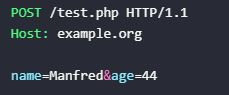
\includegraphics[scale=0.8]{includes/POST.jpg}
	\end{itemize}
	\item Werden durch \& getrennt
\end{itemize}
\end{frame}

\begin{frame}{Parameter Pollution}
\begin{itemize}[<+->]
	% \item Neben dem zu manipulierenden Parameter kann es auch einen Parameter geben der polluted wird.
	\item Einfügen oder Verändern von Parametern 
	\item Durch Manipulation existierender Parameter in codierter Form 
	\item Reservierte Zeichen in den value-strings müssen in Hexadezimalform kodiert sein 
	\begin{itemize}
		\item z.B.: \texttt{\%26} für \glqq \&\grqq{}, \texttt{\%3D} für \glqq =\grqq
	\end{itemize}
	\item So lässt sich ein \textit{\&{}name=value} Paar als \textit{\%26name\%3Dvalue} einfügen
	\item Die Parameter werden bei Benutzung des manipulierten Links dekodiert
\end{itemize}
\end{frame}

\begin{frame}{Parameter Precedence}
\begin{itemize}[<+->]
	\item Problem entsteht, wenn für einen Parameter genau ein Wert erwartet wird, aber mehrere erhalten werden
	\item Je nach Programmiersprache und Server wird unterschiedlich vorgegangen
	\item[] \begin{center}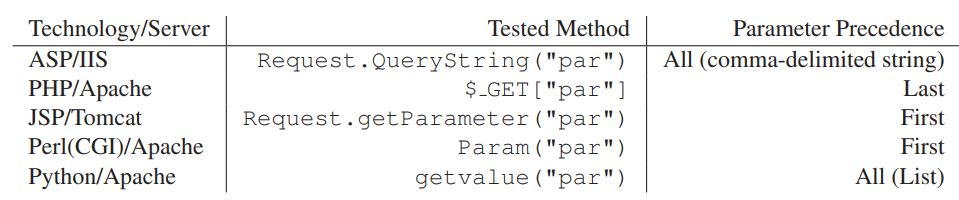
\includegraphics[scale=0.4]{includes/table1.jpg}\end{center}
	\item So können falsche Parameter in die URI hinzugefügt werden, die die Richtigen überschreiben
\end{itemize}
\end{frame}

\begin{frame}{Parameter Precedence Beispiel}
\begin{itemize}[<+->]
	\item Angenommen, es wird immer der erste Parameterwert genutzt
	\begin{itemize}
		\item[] \texttt{example.org?name=Manfred\&{}age=44}
	\end{itemize}
	\item Der erste Parameter wird \glqq polluted\grqq{}
	\begin{itemize}
		\item[] \texttt{example.org?name=Manfred\%26age\%3D20}
	\end{itemize}
	\item Wenn nun das richtige Alter eingegeben wird, werden folgende Parameter verschickt:
	\begin{itemize}
		\item[] \texttt{example.org?name=Manfred\&{}age=20\&{}age=44}
	\end{itemize}
	\item \texttt{age=44} würde ignoriert werden.
\end{itemize}
\end{frame}

\begin{frame}{Andere Formen}
\begin{itemize}%[<+->]
	\item Es können auch neue Parameter hinzugefügt werden:
	\begin{itemize} 
		\item Url: \texttt{poor.pl?par1=val1\textcolor{red!70!black}{\%26action\%3Dreset}}
		\item Link: \texttt{target.pl?x=y\&w=z\&par1=val1\textcolor{red!70!black}{\&action=reset}}
	\end{itemize}
	\item Parameter löschen durch Einfügen eines \texttt{\#}-Symbols
\end{itemize}
\end{frame}

\begin{frame}{Beispiel-Szenario}
\begin{itemize}%[<+->]
	\item Beeinflussung einer Online-Abstimmungen
	\item Wahl von zwei Kandidaten über Links
	\begin{itemize}
		\item Url: \texttt{http://host/election.jsp?\textcolor{red!70!black}{poll\_id=4568}}
		\item Link 1: \texttt{<a href="vote.jsp?\textcolor{red!70!black}{poll\_id=4568}\&\textcolor{blue!70!black}{candidate=white}">Vote for Mr. White</a>}
		\item Link 2: \texttt{<a href="vote.jsp?\textcolor{red!70!black}{poll\_id=4568}\&\textcolor{blue!70!black}{candidate=green}">Vote for Mrs. Green</a>}
	\end{itemize}
	\item \texttt{poll\_id} wird nicht richtig sanatized
\end{itemize}
\end{frame}

\begin{frame}{Beispiel-Szenario}
\begin{itemize}%[<+->]
	\item Angreifer sendet an das Opfer:
	\begin{itemize}
		\item \texttt{http://host/election.jsp?\textcolor{red!70!black}{poll\_id=4568}\textcolor{green!70!black}{\%26candidate\%3Dgreen}}
	\end{itemize}
	\item Anhand der URL werden die Links zur Wahl generiert:
	\begin{itemize} 
		\item Link 1: \texttt{<a href="vote.jsp?\textcolor{red!70!black}{poll\_id=4568}\&\textcolor{green!70!black}{candidate=green}\&\textcolor{blue!70!black}{candidate=white}">Vote for Mr. White</a>}
		\item Link 2: \texttt{<a href="vote.jsp?\textcolor{red!70!black}{poll\_id=4568}\&\textcolor{green!70!black}{candidate=green}\&\textcolor{blue!70!black}{candidate=green}">Vote for Mrs. Green</a>}
	\end{itemize}
	\item Es werden immer zwei Parameter \texttt{candidate} übergeben
	\item Nur der erste Parameter wird verwendet
	\item Mrs. Green wird immer gewählt
\end{itemize}
\end{frame}

\begin{frame}{Häufigkeit}
\begin{itemize}%[<+->]
	\item Paper von Balduzzi et al. (2011) untersucht ca. 5000 Websites
	\begin{itemize}
		\item PAPAS tool (PArameter Pollution Analysis System)
		\item Sucht nach Client-side vulnerabilities
		\item Test auf Parameter Precedence und Injection von Parametern per URL-Encoding
	\end{itemize}
	\item $30\%$ hatten HPP vulnerabilities
	\begin{itemize}
		\item davon waren min. $46.8\%$ exploitable
		\item Unabhängig von Kategorie der Website
	\end{itemize}
	\item Auch bekannte Websites (Google, Microsoft) darunter
	\item Aktuellere Untersuchungen nicht bekannt
\end{itemize}
\end{frame}

\begin{frame}{Gefundene Beispiele}
\begin{itemize}%[<+->]
\item Integrierter share-Button von sozialen Netzwerken
	\begin{itemize}
		\item z.B. auf Nachrichtenseiten
		\item[] 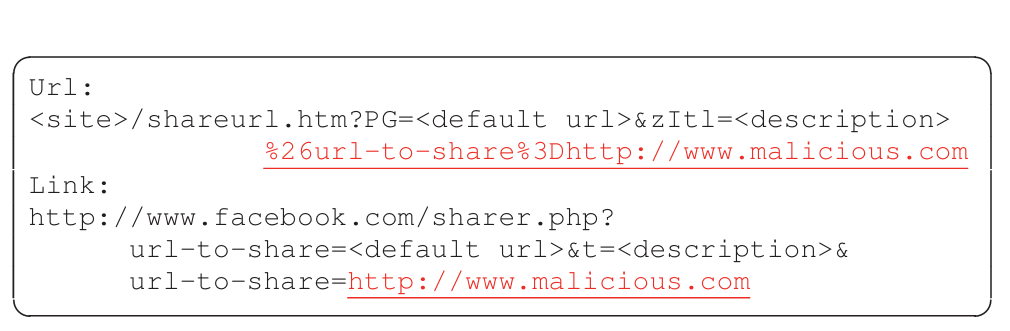
\includegraphics[scale=0.35]{includes/sharegrafik.png}
	\end{itemize}
\item \glqq Einkaufskorb\grqq{} auf Shopping-Seiten
	\begin{itemize}
		\item Items konnten hinzugefügt oder geändert werden
	\end{itemize}
	\item Banking-Webseiten
	\item Filtereinstellungen auf verschiedenen Webseiten
\end{itemize}
\end{frame}

\begin{frame}{Gegenmaßnahmen}
\begin{itemize}%[<+->]
	\item Input sanitation
	\item Nur bekannte Parameter akzeptieren
	\item Parameter nur dort akzeptieren, wo sie erwartet werden
	\item Berücksichtigung von doppelten Parametern
\end{itemize}
\end{frame}

\end{document}
